\documentclass[12pt]{article}
\usepackage{geometry}
 \geometry{
 a4paper,
 total={170mm,257mm},
 left=20mm,
 top=20mm,
 }
\usepackage{amsmath}
\usepackage{amssymb}
\usepackage{graphicx}
\usepackage{hyperref}
\usepackage{cleveref}
\usepackage[most]{tcolorbox}
\usepackage[utf8]{inputenc}
\usepackage{tikz}
\usepackage{pstricks-add}
\usepackage{mathtools}
\usetikzlibrary{arrows,calc}
\title{MAT 1001: Calculus I}
\author{Alfonsus Rodriques Rendy}
\date{2021-9-7}

\begin{document}
\begin{center}
    \hspace*{-0.5cm}
    \framebox{
    \begin{minipage}{1\linewidth}
        \textbf{MAT1001 Calculus I} \\
        \vspace{-0.8cm}
        \begin{center}
            \huge{Lecture 1 : Introduction to Calculus} 
            \\
            \vspace{0.5cm}
            \normalsize \textit{Lecture by Dr. Arjan Abeynaike} \\
            \vspace{0.3cm}
            \text{Scribe by Alfonsus Rodriques Rendy} \\
            \textrm{Sep 7, 2021}
        \end{center}
    \end{minipage}}
\end{center}

\section{Introduction}
\paragraph{What is calculus?} Calculus is the study how things change. It provides us a toll to model changes that happen around us.

\section{Mathematical Background: Set}
\subsection{Definition}
A set is a collection of distinct objects; these objects are called
elements of the set. Some definition and notation of sets:
\begin{itemize}
    \item $x \in S$ means $x$ is an element of the set $S$"; we say that $x$ belongs to ,$S$ or simply $x$ is in $S$.
    \item $x \notin S$ means $x$ is not an element of $S$".
    \item $S \subseteq T$ means every element of $S$ is an element of $T$"; we say that $S$ is a subset of $T$, or that $S$ is contained in $T$.
    \item $S = T$ means that $S \subseteq T$ and $T \subseteq S$ both hold.
    \item $S \subsetneq T$ means that $S \subseteq T$ and $S \neq T$ (we say that $S$ is a proper subset of $T$).
    \item $ \emptyset $ denotes the set containing no element (called the empty set).
\end{itemize}

\noindent
We use $\{x \subseteq S : P(x)\} \textrm{ or } \{x \subseteq S \mid P(x)\} $ to denote the set of all elements $x$ in $S$ for which $P(x)$ is true. 
We may simply write $\{x : P(x)\} $ when $S$ is obvious or not important.
The following symbols are frequently used:
\begin{itemize}
    \item $ \mathbb{Z} := \{..., 0, 1, 2, ...\} $ is the set of integers.
    \item $ \mathbb{N} := \{n \in \mathbb{Z} : n \geq 2\} = \{..., 0, 1, 2, 3, ...\}$ is the set of natural numbers.
    \item $ \mathbb{N_+} := \{n \in \mathbb{Z} : n > 2\} = \{..., 1, 2, 3, ...\}$ is the set of positive integers.
    \item $ \mathbb{Q} := \{m/n : m \in Z, n \in N_+\} $ is the set of rational numbers.
    \item $ \mathbb{R} $ is the set of real numbers.
\end{itemize}

\paragraph{Note} We use the symbol := to mean that the symbol on the left is defined by the object on the right.

\subsection{Set Operations}
\noindent 
Let $S$ and $T$ be sets. We define:
\begin{itemize}
    \item $S \cap T := \{x : x \in S \textrm{ and } x \in T \} $ (Intersection of $S$ and $T$)
    \item $S \cup T := \{x : x \in S \textrm{ or } x \in T \} $ (Union of $S$ and $T$)
    \item $S \setminus T := \{x : x \in S \textrm{ and } x \notin T \} $ ($S$ minus $T$). It is also common to write $S - T$ instead of $S \setminus T$.
\end{itemize}
\noindent
$ \mathbb{R} \setminus \mathbb{Q} $, the set of all real numbers that are not rational, is
called the set of irrational numbers. Examples of irrational numbers include $\pi, \sqrt{2}, \textrm{ and } e $ \\
If $ S \cap T = \emptyset $, then we say that $S$ and $T$ are disjoint.

\subsection{Cartesian Products}
\paragraph{Definition} 
Let $S$ and $T$ be nonempty sets. The Cartesian product of $S$ and
$T$, denoted by $S \times T$, is the set of all ordered pairs $(x, y)$ such
that $x \in S$ and $y \in T$. That is,
\[S \times T := \{(x, y) : x \in S, y \in T\} \]

\noindent
More generally, if $S_1, ...,  S_n$ are nonempty sets, the Cartesian
product of $S_1, ..., S_n$ is defined to be
\[S_1 \times ... \times S_n := \{(x_1, ..., x_n) : x_1 \in S_1, ... , x_n \in S_n\} \]
An object of the form $(x_1, ... , x_n)$ is called an (ordered) n-tuple.

If $S = \{1, 2, 3\} \textrm{ and } T = \{4, 8\} $ then
\[S \times T = \{(1, 4), (1, 8), (2, 4), (2, 8), (3, 4), (3, 8)\} \]

We use the symbol $S_n$ to mean $S \times \textrm{ ... } \times S$ (with $n$ copies of
$S$). In particular, $\mathbb{R}^2$ is the set of all ordered pairs of real
numbers:
\[\mathbb{R}^2 := \mathbb{R} \times \mathbb{R} = \{(x, y) : x \in \mathbb{R}, y \in \mathbb{R}\} \]
Similarly, $R^n$ is the set of all ordered n-tuples of real numbers.

\subsection{Interval}
We use the following notations for intervals, where $a \in \mathbb{R}$ and
$b \in \mathbb{R}$:
\begin{itemize}
    \item $[a, b] :=\{x \in \mathbb{R} : a \leq x \leq b \}$ (Closed intervals)
    \item $(a, b) :=\{x \in \mathbb{R} : a < x < b \}$ (Open intervals)
    \item $[a, b):=\{x \in \mathbb{R} : a \leq x < b \}$ (Half-open or half-closed intervals)
    \item $(a, b]$ is defined similarly.
\end{itemize}

\noindent
We also allow $a$ or $b$ to be $\infty$ or $-\infty$ for unbounded intervals. 
For example: 
\[(-\infty, \infty) := \mathbb{R} \] 
\[[0, \infty) := \{x \in \mathbb{R} : x \geq 0 \}\].

\section{Function}
\subsection{Definition}
\begin{figure}[h!]
    \centering
    \includegraphics[width=0.7\linewidth]{images/function.png}
    \caption{Function illustration}
    \label{fig:function}
\end{figure}
A function is like a "machine" that takes input x which then go into a defined process 
resulted in output $f(x)$.
A function consists of three objects, that is:
\begin{itemize}
    \item A non empty set D, called the domain;
    \item A non empty set Y, called the codomain;
    \item A rule, $f$ such that, for each element $x_0 \in D$ , $f$ assigns
          exactly one element in $Y$ to $x_0$; this element is denoted by $f(x)$
\end{itemize}
\paragraph{Definition} A function from $D$ to $Y$ is a rule that assigns to each element
of $D$ exactly one element of $Y$. We use the notation $ f : D \rightarrow Y $ to mean that the function $f$ is
from $D$ to $Y$, with $f(x)$ being the element of $Y$ assigned to $x$.
For a function $f : D \rightarrow Y $ , the set $D$ and $Y$ are called the
domain and the codomain of $f$, respectively, and the set $\{f(x) : x \in D \} $ is called the range of $f$.

\paragraph{Note} If $x$ and $y$ are variables related by $y = f(x)$, $x$ is called the independent variable and
$y$ is called the dependent variable
\subsection{Piecewise Function}
\paragraph{Definition} A piecewise function is a function built from pieces of different functions over different intervals. \\
A function may be defined piecewisedly, for example,
\[
f(x) = 
\begin{cases}
    2x + 1 & 0 \leq x \leq 3 \\
    \sqrt{x + 6} & 3 < x < 10 \\
\end{cases}
\]
$f(x)$ can be denoted as $f : [0, 10) \rightarrow \mathbb{R} $ with $ [0, 10) = \{x : 0 \leq x < 10\} $

\section{Rate of Change}
\subsection{Average Rate of Change}
\paragraph{Definition} For $y = f(x)$ the average rate of change of $y$ with respect to $x$ from $x = x_1$ to $x = x_2$ is 
\[
    \frac{\Delta y}{\Delta x} = \frac{f(x_2) - f(x_1)}{x_2 - x_1} = \frac{f(x_1 + \epsilon) - f(x_1)}{\epsilon}
\]
\begin{center}
    where $\epsilon = \Delta x = x_2 - x_1$
\end{center}
\paragraph{Geometric Representation} Average rate of change is related to \textbf{secant line}. 
Secant line on a curve $f$ is a line joining two points of the curve $f$. The slope of a secant line
is the average rate of change between two point intersection of secant line and the curve.

\vspace*{1cm}

\begin{figure}[h!]
\centering
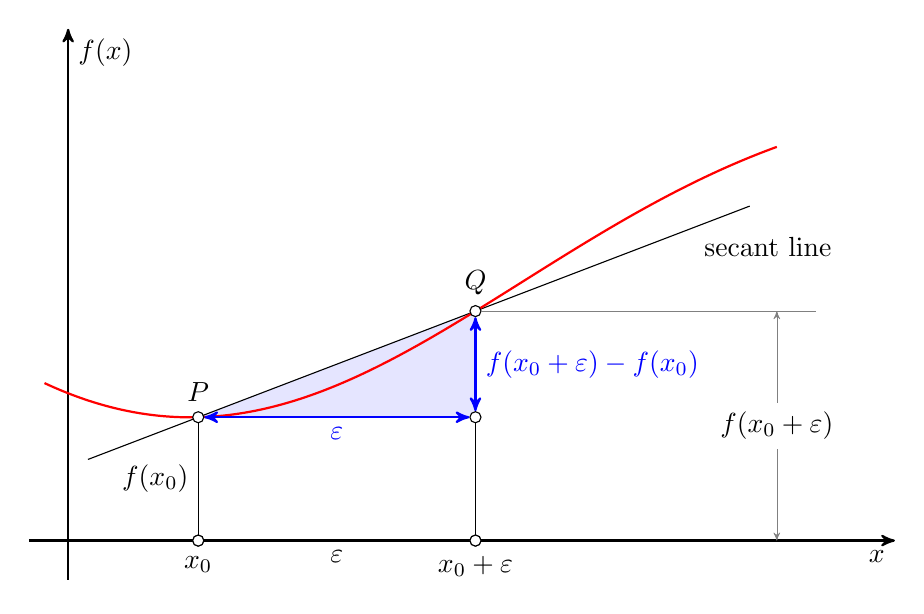
\begin{tikzpicture}[>=stealth',
    dot/.style={circle,draw,fill=white,inner sep=0pt,minimum size=4pt}]

% draw axis lines
\draw[->,thick] (-0.5,0) -- ++(11,0) node[below left]{$x$};
\draw[->,thick] (0,-0.5) -- ++(0,7) node[below right]{$f(x)$};
\coordinate (O) at (0,0);

% create path for function curve
\path[thick,red] (-0.3,2) to[out=-25, in=200] coordinate[pos=0.2] (p) coordinate[pos=0.6] (q) (9,5);
% fill area
\fill[blue, opacity=.1] (p) -| (q);
% draw the secant line with fixed length
\draw[shorten <=-1.5cm] (p) -- ($ (p)!7.5cm!(q) $) node[below right, pos=0.9]{secant line};
% draw function curve
\draw[thick,red] (-0.3,2) to[out=-25, in=200] (9,5);

% draw all points
\node[dot,label={above:$P$}] (P) at (p) {};
\node[dot,label={above:$Q$}] (Q) at (q) {};
\node[dot] (p1) at (P |- O) {};
\node[dot] (p2) at (Q |- O) {};
\node[dot] (p3) at (P -| Q) {};

% draw lines between nodes and place text
\draw (P) -- node[left]{$f(x_{0})$} (p1) node[dot,label={below:$x_{0}$}]{};
\draw (p2) node[dot,label={below:$x_{0} + \varepsilon$}]{} -- (p3);
\path (p1) -- node[below]{$\varepsilon$} (p2);

% draw blue arrows between nodes
\draw[<->,blue,thick] (P) -- node[below]{$\varepsilon$} (p3);
\draw[<->,blue,thick] (Q) -- node[right]{$f(x_{0} + \varepsilon) - f(x_{0})$} (p3);

% draw the explanation for the y-value of point Q
\draw[help lines] (Q) -- (Q -| {(9.5,0)}) ++(-0.5,0) coordinate (p4);
\draw[help lines, <->] (p4) -- node[fill=white,text=black]{$f(x_{0} + \varepsilon)$} (p4 |- O);

\end{tikzpicture}
\caption{Illustration of secant line}
\end{figure}

\noindent
The slope of the secant line through P and Q $ = \Delta f(x) / \Delta x $
which is the average rate of change with respect to $x$ over $[x_0, x_0 + \epsilon]$

\subsection{Instataneous Rate of Change}
\paragraph{Definition} The instantaeous rate of change is the change in the rate at a particular instant. 
We can find the of instantaneous rate of change at $x_0$ by using average of rate of change over $[x_0, x_1]$ with
$x_1$ "very close" to $x_0$. \\
\noindent
For example:
\[
    \textrm{Let }y = f(x) = t^2 \textrm{ , } x_0 = 1
\]
\begin{center}
    \begin{tabular}{|c|c|c|c|c|c|c|}
        \hline
        $x_1$ & 0.9 & 0.99 & 0.999 & 1.001 & 1.01 & 1.1 \\
        \hline
        $\frac{f(x_1) - f(x_0)}{x_1 - x_0}$ & 1.9 & 1.99 & 1.999 & 2.001 & 2.01 & 2.1\\
        \hline
    \end{tabular}
\end{center}

As $x_1$ approach $x_0 = 1$, the value of the average of change of y is getting closer to 2.
Therefore, we can denote the instantaneous rate of change as:
\[
    \lim_{x_1 \to x_0} \frac{f(x_1) - f(x_0)}{x_1 - x_0} = \lim_{\Delta x \to 0} \frac{\Delta y}{\Delta x}
\]

\paragraph{Geometric Representation} While average rate of change is related to secant line, instantaneous rate of change
is related to \textbf{tangent line}. Tangent line of a curve $f$ at $x_0$ is a line that just "touches" the curve $f$ at 
point $x_0$

\vspace*{0.5cm}

\begin{figure}[h!]
\centering
    \begin{tikzpicture}
        \draw[->] (-0.5, 0) -- (9, 0) node[right] {$x$};
        \draw[->] (0, -0.5) -- (0, 5) node[above] {$y$};
        \draw[scale=1, domain=0:8, smooth, variable=\x, red] plot ({\x}, {0.1*\x^2 - 0.6*\x + 2.1}) node[above] {$y = f(x)$};
        \draw[dashed] (6,2.1) -- (6,0) node[below] {$x_0$};
        \filldraw [draw=black, fill=white] (6,2.1) circle (2pt) node[above] {$P$};
        \draw[thick] (2.5,0) -- (7.5, 3) node[right] {Tangent Line};
    \end{tikzpicture}
    \caption{Illustration of tangent line}
\end{figure}
\noindent
Slope of a tangent line at point $x_0$ is the instantaneous rate of change at point $x_0$.
In other words, it is the limit of the slope of the secant line as x approaches $x_0$.
\paragraph{Example} Let a function of the position of an object denoted as 
\[
    f(x) = x^2 
\]
What is the tangent line at $x = 1$? \\ \\
Let $t$ be an arbitrarily point that is close to 1. Therefore, we have the slope of the secant line $L_t$
\[
    L_t = \frac{t^2 - 1^2}{t - 1} 
\]
To get the instantaneous rate of change or the slope of the tangent line, we take the limit of the slope
of the secant line as $t$ approaches 1, that is
\[
    \lim_{t \to 1} \frac{t^2 - 1}{t - 1}\, = \lim_{t \to 1} \frac{(t - 1)(t + 1)}{t - 1} = t + 1
\]
Hence, we have the slope of the tangent line at $t=1$ is $t + 1 =  2$.\\
The equation of the tangent line is

\begin{align*}
    \frac{y - 1^2}{x - 1} &= 2 \\
    y &= 2x - 1
\end{align*}
\paragraph{Note}
Average rate of change is the same slope of secant line, and 
instantaneous rate of change is the same slope of tangent line
\end{document}
